\documentclass[8pt,a4paper]{article}

\usepackage{amsmath, amssymb, amsthm,stackengine}
\usepackage{tikz}
\usepackage{mathtools}
\usepackage{multicol}
\usepackage[top=0.5cm,left=0.5cm,right=0.5cm,bottom=0.5cm]{geometry}
\usepackage{amsfonts}
\usepackage{etoolbox}
\usepackage{cancel}
\usepackage{yhmath}
\usepackage{color}
\usepackage{hyperref}
\usepackage{cancel}
\usepackage{graphicx}
\usepackage{caption}
\usepackage[overload]{empheq} % For braced-style systems of equations.

\usepackage{bm}
\usepackage{centernot}
\usepackage{tikz}
\newcommand{\circled}[1]{%
  \tikz[baseline=(char.base)]\node[shape=circle,draw,inner sep=2pt] (char) {#1};%
}

%\usepackage[mathabx]{mathabx}

% Declare necessary fonts from mathabx
\DeclareFontFamily{U}{matha}{\hyphenchar\font45}
\DeclareFontShape{U}{matha}{m}{n}{
  <-6> matha5 <6-7> matha6 <7-8> matha7
  <8-9> matha8 <9-10> matha9
  <10-12> matha10 <12-> matha12
}{}
\DeclareSymbolFont{matha}{U}{matha}{m}{n}

% Declare necessary fonts from mathabx
\DeclareFontFamily{U}{mathb}{\hyphenchar\font45}
\DeclareFontShape{U}{mathb}{m}{n}{
  <-6> mathb5 <6-7> mathb6 <7-8> mathb7
  <8-9> mathb8 <9-10> mathb9
  <10-12> mathb10 <12-> mathb12
}{}
\DeclareSymbolFont{mathb}{U}{mathb}{m}{n}

\DeclareMathSymbol{\coloneq}       {3}{mathb}{"15}
\DeclareMathSymbol{\eqcolon}       {3}{mathb}{"16}
\DeclareMathSymbol{\subsetneqq}    {3}{matha}{"90}
\DeclareMathSymbol{\nLeftarrow}    {3}{matha}{"F6}

\newcommand{\impliesnotimplied}{%
  \mathrel{%
    \vcenter{\offinterlineskip
      \ialign{##\cr$\nLeftarrow$\cr\noalign{\kern+1pt}$\Rightarrow$\cr}%
    }%
  }%
}

\newenvironment{Figure}
  {\par\medskip\noindent\minipage{\linewidth}}
  {\endminipage\par\medskip}

\definecolor{forestgreen(web)}{rgb}{0.13, 0.55, 0.13}
\definecolor{lavender(floral)}{rgb}{0.71, 0.49, 0.86}

\usepackage{nicefrac, xfrac}
%\usepackage{mathtools}
\newcommand{\abs}[1]{\left\lvert #1 \right\rvert}
\newcommand{\norm}[1]{\left\lVert #1 \right\rVert}
\newcommand{\sca}[1]{\left\langle #1 \right\rangle}

\newcommand{\dualH}[4]{{}_{_{H^{\resizebox{0.5\width}{0.5\height}{#2}}}}\!\langle #1 \rangle\!{}_{_{H^{\resizebox{0.5\width}{0.5\height}{#3}}_{\resizebox{0.5\width}{0.5\height}{#4}}}}}

\newcommand{\dualHv}[1]{{}_{_{\mathbf{H}'}}\!\langle #1 \rangle{}_{_{\mathbf{V}\subset\mathbf{H}}}}

\newcommand{\dualVv}[1]{{}_{_{\mathbf{V}'}}\!\langle #1 \rangle{}_{_{\mathbf{V}}}}

\newcommand{\dualT}[3]{{}_{_{H^{\resizebox{0.5\width}{0.5\height}{#2}}}}\!\langle #1 \rangle\!{}_{_{H^{\resizebox{0.5\width}{0.5\height}{#3}}}}}

\newcommand{\dualV}[3]{{}_{_{\mathbf{#2}^{\resizebox{0.5\width}{0.5\height}{#3}}}}\!\langle #1 \rangle{}_{_{\mathbf{V}}}}


%\usepackage{xcolor}
\usepackage{titlesec}

%\usepackage{wasysym}
%\smiley{}

\usepackage{tikzsymbols}


% Bold
\renewcommand{\AA}{\mathbb A}
\newcommand{\BB}{\mathbb{B}}
\newcommand{\CC}{\mathbb{C}}
\newcommand{\DD}{\mathbb{D}}
\newcommand{\EE}{\mathbb{E}}
\newcommand{\FF}{\mathbb{F}}
\newcommand{\GG}{\mathbb{G}}
\newcommand{\HH}{\mathbb{H}}
\newcommand{\II}{\mathbb{I}}
\newcommand{\JJ}{\mathbb{J}}
\newcommand{\KK}{\mathbb{K}}
\newcommand{\LL}{\mathbb{L}}
\newcommand{\MM}{\mathbb{M}}
\newcommand{\NN}{\mathbb{N}}
\newcommand{\OO}{\mathbb{O}}
\newcommand{\PP}{\mathbb{P}}
\newcommand{\QQ}{\mathbb{Q}}
\newcommand{\RR}{\mathbb{R}}
\renewcommand{\SS}{\mathbb S}
\newcommand{\TT}{\mathbb{T}}
\newcommand{\UU}{\mathbb{U}}
\newcommand{\VV}{\mathbb{V}}
\newcommand{\WW}{\mathbb{W}}
\newcommand{\XX}{\mathbb{X}}
\newcommand{\YY}{\mathbb{Y}}
\newcommand{\ZZ}{\mathbb{Z}}

% Calligraphic
\newcommand{\Ac}{\mathcal{A}}
\newcommand{\Bc}{\mathcal{B}}
\newcommand{\Cc}{\mathcal{C}}
\newcommand{\Dc}{\mathcal{D}}
\newcommand{\Ec}{\mathcal{E}}
\newcommand{\Fc}{\mathcal{F}}
\newcommand{\Gc}{\mathcal{G}}
\newcommand{\Hc}{\mathcal{H}}
\newcommand{\Ic}{\mathcal{I}}
\newcommand{\Jc}{\mathcal{J}}
\newcommand{\Kc}{\mathcal{K}}
\newcommand{\Lc}{\mathcal{L}}
\newcommand{\Mc}{\mathcal{M}}
\newcommand{\Nc}{\mathcal{N}}
\newcommand{\Oc}{\mathcal{O}}
\newcommand{\Pc}{\mathcal{P}}
\newcommand{\Qc}{\mathcal{Q}}
\newcommand{\Rc}{\mathcal{R}}
\newcommand{\Sc}{\mathcal{S}}
\newcommand{\Tc}{\mathcal{T}}
\newcommand{\Uc}{\mathcal{U}}
\newcommand{\Vc}{\mathcal{V}}
\newcommand{\Wc}{\mathcal{W}}
\newcommand{\Xc}{\mathcal{X}}
\newcommand{\Yc}{\mathcal{Y}}
\newcommand{\Zc}{\mathcal{Z}}

% Bold Big Vector
\newcommand{\Av}{\mathbf{A}}
\newcommand{\Bv}{\mathbf{B}}
\newcommand{\Cv}{\mathbf{C}}
\newcommand{\Dv}{\mathbf{D}}
\newcommand{\Ev}{\mathbf{E}}
\newcommand{\Fv}{\mathbf{F}}
\newcommand{\Gv}{\mathbf{G}}
\newcommand{\Hv}{\mathbf{H}}
\newcommand{\Iv}{\mathbf{I}}
\newcommand{\Jv}{\mathbf{J}}
\newcommand{\Kv}{\mathbf{K}}
\newcommand{\Lv}{\mathbf{L}}
\newcommand{\Mv}{\mathbf{M}}
\newcommand{\Nv}{\mathbf{N}}
\newcommand{\Ov}{\mathbf{O}}
\newcommand{\Pv}{\mathbf{P}}
\newcommand{\Qv}{\mathbf{Q}}
\newcommand{\Rv}{\mathbf{R}}
\newcommand{\Sv}{\mathbf{S}}
\newcommand{\Tv}{\mathbf{T}}
\newcommand{\Uv}{\mathbf{U}}
\newcommand{\Vv}{\mathbf{V}}
\newcommand{\Wv}{\mathbf{W}}
\newcommand{\Xv}{\mathbf{X}}
\newcommand{\Yv}{\mathbf{Y}}
\newcommand{\Zv}{\mathbf{Z}}

% Bold Little Vector
\newcommand{\av}{\mathbf{a}}
\newcommand{\bv}{\mathbf{b}}
\newcommand{\cv}{\mathbf{c}}
\newcommand{\dv}{\mathbf{d}}
\newcommand{\ev}{\mathbf{e}}
\newcommand{\fv}{\mathbf{f}}
\newcommand{\gv}{\mathbf{g}}
\newcommand{\hv}{\mathbf{h}}
\newcommand{\iv}{\mathbf{i}}
\newcommand{\jv}{\mathbf{j}}
\newcommand{\kv}{\mathbf{k}}
\newcommand{\lv}{\mathbf{l}}
\newcommand{\mv}{\mathbf{m}}
\newcommand{\nv}{\mathbf{n}}
\newcommand{\ov}{\mathbf{o}}
\newcommand{\pv}{\mathbf{p}}
\newcommand{\qv}{\mathbf{q}}
\newcommand{\rv}{\mathbf{r}}
\newcommand{\sv}{\mathbf{s}}
\newcommand{\tv}{\mathbf{t}}
\newcommand{\uv}{\mathbf{u}}
\newcommand{\vv}{\mathbf{v}}
\newcommand{\wv}{\mathbf{w}}
\newcommand{\xv}{\mathbf{x}}
\newcommand{\yv}{\mathbf{y}}
\newcommand{\zv}{\mathbf{z}}

\renewcommand{\hat}{\widehat}

% differenziale
\newcommand{\dspace}{\ } % \, aggiunge un piccolo spazio
\newcommand{\de}{\mathrm{d}}
\newcommand{\dx}{\dspace \de x}
\newcommand{\dy}{\dspace \de y}
\newcommand{\dt}{\dspace \de t}
\newcommand{\dS}{\dspace \de S}
\newcommand{\ds}{\dspace \de s}
\newcommand{\dz}{\dspace \de z}
\newcommand{\dw}{\dspace \de w}
\newcommand{\du}{\dspace \de u}
\newcommand{\dvv}{\dspace \de v}
\newcommand{\db}{\dspace \de b}
\newcommand{\dteta}{\dspace \de \vartheta}
\newcommand{\dxi}{\dspace \de \xi}
\newcommand{\dxy}{\dspace \de x \de y}
\newcommand{\duv}{\dspace \de u \de v}
\newcommand{\dst}{\dspace \de s \de t}
\newcommand{\dP}{\dspace \de P}
\newcommand{\dPP}{\dspace \de \PP}
\newcommand{\dsig}{\dspace \de \sigma}
\newcommand{\dth}{\dspace \de \theta}
\newcommand{\deta}{\dspace \de \eta}
\newcommand{\dph}{\dspace \de \varphi}
\newcommand{\dxv}{\dspace \de \mathbf{x}}
\newcommand{\dSx}{\dspace \de \text{S}(x)}

\newcommand{\Bot}{\perp \!\!\! \perp} % indipendenza
\usepackage{dsfont} % per funzione indicatrice
\newcommand{\Ind}{\mathds{1}} % funzione indicatrice

\DeclareMathOperator{\Det}{det} % determinante
\DeclareMathOperator{\Img}{Im}
\DeclareMathOperator{\Ker}{Ker}
\DeclareMathOperator{\ArgMin}{ArgMin}
\DeclareMathOperator*{\esssup}{ess\,sup}
\DeclareMathOperator{\Div}{div}
\newcommand{\nabladot}{\nabla\!\!\cdot\!}
\DeclareMathOperator{\Lip}{Lip}

\renewcommand{\theta}{\vartheta}

%\DeclareMathOperator{\ker}{ker}
 
 % Turn off header and footer
\pagestyle{empty}

% Redefine section commands to use less space
\makeatletter
\newcommand{\chapter}{\@startsection{chapter}{1}{0mm}%
                                {-0.1ex plus -.5ex minus -.2ex}%
                                {1.5ex plus .2ex}%x
                                {\center\normalfont\Huge\bfseries\color{teal}}}
\renewcommand{\section}{\@startsection{section}{1}{0mm}%
                                {-0.1ex plus -.5ex minus -.2ex}%
                                {1.5ex plus .2ex}%x
                                {\center\normalfont\large\bfseries\color{forestgreen(web)}}}
\newcommand{\FSIsection}{\@startsection{section}{1}{0mm}%
                                {-0.1ex plus -.5ex minus -.2ex}%
                                {1.5ex plus .2ex}%x
                                {\center\normalfont\large\bfseries\color{red}}}
\renewcommand{\subsection}{\@startsection{subsection}{2}{0mm}%
                                {-0.1ex plus 0ex minus 0ex}%
                                {1.5ex plus 0ex}%
                                {\normalfont\scriptsize\bfseries\color{red}}}
\newcommand{\FSIsubsection}{\@startsection{subsection}{2}{0mm}%
                                {-0.1ex}%
                                {1ex}%
                                {\normalfont\scriptsize\bfseries\color{red}}}
\renewcommand{\subsubsection}{\@startsection{subsubsection}{3}{0mm}%
                                {-1ex plus -.5ex minus -.2ex}%
                                {1ex plus .2ex}%
                                {\normalfont\small\bfseries}}
\makeatother

\titlespacing\section{0pt}{0pt plus 0pt minus 0pt}{0pt plus 0pt minus 0pt}

% Don't print section numbers
\setcounter{secnumdepth}{0}

\setlength{\parindent}{0pt}
\setlength{\parskip}{0pt plus 0ex}

% -----------------------------------------------------------------------

\begin{document}

\raggedright
\footnotesize
\begin{multicols*}{3}

% multicol parameters
% These lengths are set only within the two main columns
%\setlength{\columnseprule}{0.25pt}
\setlength{\premulticols}{1pt}
\setlength{\postmulticols}{1pt}
\setlength{\multicolsep}{1pt}
\setlength{\columnsep}{2pt}

%!TEX root = ../main.tex

% =================================================
% =================================================

\section{\texorpdfstring{\color{forestgreen(web)}Hilbertian Sobolev Spaces}{}}

% =================================================
% =================================================

% =================================================

\subsection{\texorpdfstring{\color{red}Sobolev Space \texorpdfstring{$H^1$}{C} in dim. \texorpdfstring{$n=1$}{C}}{}}

% =================================================

$u\in L^2(a,b)$ admits weak derivative if $\exists\,g\in L^2(a,b)$ s.t.
\begin{equation*}
\int_a^b u\,\varphi'=-\int_a^b g\,\varphi\quad\forall\, \varphi\in \Dc(a,b)
\end{equation*}
If so, $u':=g$.

\rule{0.31\textwidth}{0.2pt}
\smallskip

$H^1(a,b) = \left\{ u\in L^2(a,b),\ u'\in L^2(a,b) \right\}$

\rule{0.31\textwidth}{0.2pt}
\smallskip

$\Cc^1([a,b])\subset H^1(a,b)$ (weak derivative $\equiv$ classic)

\rule{0.31\textwidth}{0.2pt}
\smallskip

$H^1(a,b)$ endowed with
\begin{align*}
(u,v)_{H^1}&=(u,v)_{L^2}+(u',v')_{L^2} \\
\norm{u}_{H^1}&=\left( \norm{u}^2_{L^2}+\norm{u'}^2_{L^2} \right)^{1/2}
\end{align*}

is an Hilbert separable space.

\rule{0.31\textwidth}{0.2pt}
\smallskip

$\norm{u}_{*}=\norm{u}_{L^2}+\norm{u'}
_{L^2}$ is an equivalent norm.

\rule{0.31\textwidth}{0.2pt}
\smallskip

\textbf{Thm (Embedding).} $\forall\,u\in H^1(I)$, $\exists\,\widetilde{u}\in\Cc^0(\overline{I})$ s.t. $u=\widetilde{u}$ a.e. on $I$ and 
\begin{equation*}
\widetilde{u}(x)-\widetilde{u}(y)=\int_x^y u'(t)\dt\qquad\forall\, x,y\in \overline{I}
\end{equation*}
$\hookrightarrow$ $u$ admits a continuous representative!

\rule{0.31\textwidth}{0.2pt}
\smallskip

$H^1_0(I):=\overline{\Dc(I)}^{H^1}$, it is a separable Hilbert space if endowed with the inner product induced by $H^1(I)$. If $I=\RR$ then $H^1_0(\RR)=H^1(\RR)$, otherwise if $I\subset\RR$ then $H^1_0(I)$ is a proper closed subspace of $H^1(I)$, and it's characterized by:

\smallskip

\textbf{Thm.} $I\neq\RR$, $u\in H^1(I)$. $u\in H^1_0(I)$ $\Leftrightarrow$ $u\big|_{\partial I}=0$

\rule{0.31\textwidth}{0.2pt}
\smallskip

\textbf{Thm (Poincaré inequality).} $\forall\, u\in H^1_0(a,b)$
\begin{equation*}
\norm{u}_{L^2}\leq (b-a)\cdot \norm{u'}_{L^2}
\end{equation*}

\textbf{\color{lavender(floral)}Proof.} See whiteboards u.u

\smallskip

Thanks to this: on $H^1_0$ the norms $\norm{u}_{H^1}$ and $\norm{u'}_{L^2}$ are equivalent.

\rule{0.31\textwidth}{0.2pt}
\smallskip

$H^{-1}(I):=\left[ H^1_0(I) \right]'$, if we identify $L^2$ with its dual using Riesz Representation Thm., then we have the following \textbf{Hilbert triplet}:
\begin{equation*}
H_0^1(I)\subset L^2(I) \subset H^{-1}(I)
\end{equation*}

The embedding should be understood as: $\forall\, u\in L^2(I)$ we associate the functional $T_u\in H^{-1}(I)$ defined by
\begin{equation*}
\sca{T_u,v}:=\int_I u\,v\qquad \forall\, v\in H^1_0(I)
\end{equation*}

\rule{0.31\textwidth}{0.2pt}
\smallskip

\textbf{Thm.} $F\in H^{-1}(I)$ $\Rightarrow$ $\exists\ f_0,f_1\in L^2(I)$ s.t.
\begin{equation*}
\sca{F,u}=\int_I f_0\,u+\int_I f_1\,u'\quad\forall\,u\in H^1_0(I)
\end{equation*}
If $I=(a,b)$ then you can take $f_0=0$.

\medskip

$\hookrightarrow$ In the bdd case, the thm  states that 
\begin{equation*}
\sca{F,\varphi}=\int_a^b f_1\,\varphi'=-\sca{f_1',\varphi}\quad \forall\, \varphi\in\Dc'(a,b)
\end{equation*}
i.e. $-F$ is the distributional derivative of $f_1\in L^2(a,b)$, thus elements in $H^{-1}(a,b)$ have "-1 derivatives" in $L^2(a,b)$.

\smallskip

\textcolor{blue}{\underline{ex}: Dirac Delta}

\rule{0.31\textwidth}{0.2pt}

% =================================================

\subsection{\texorpdfstring{\color{red}Sobolev Spaces \texorpdfstring{$H^k,\ k\in\NN,$}{C} in dim. \texorpdfstring{$n=1$}{C}}{}}

% =================================================

Let's start with $k=2$. We have:
\begin{align*}
H^2(I)&=\left\{ u\in H^1(I),\ u'\in H^1(I) \right\}\\&=\left\{ u,u',u''\in L^2(I) \right\}
\end{align*}
endowed with
\begin{align*}
(u,v)_{H^2}&=(u,v)_{L^2}+(u',v')_{L^2}+(u'',v'')_{L^2} \\
\norm{u}^2_{H^2}&=\norm{u}_{L^2}^2+\norm{u'}_{L^2}^2+\norm{u''}_{L^2}^2
\end{align*}

\rule{0.31\textwidth}{0.2pt}
\smallskip

\textbf{Thm (Embedding).} $\forall\,u\in H^2(I)$, $\exists\,\widetilde{u}\in\Cc^1(\overline{I})$ s.t. $u=\widetilde{u}$ a.e. on $I$

\smallskip

$\hookrightarrow$ $u$ admits a differentiable representative!

\rule{0.31\textwidth}{0.2pt}

\newcolumn 

$
H^2_0(I):=\overline{\Dc(I)}^{H^2}
$ \\
$\qquad\quad\overset{\text{thm}}{=}\left\{ u\in H^2(I)\ :\ u\big|_{\partial I}=u'\big|_{\partial I}=0 \right\}
$

\rule{0.31\textwidth}{0.2pt}
\smallskip

\textbf{Thm (Poincaré inequality).} $\forall\, u\in H^2\cap H^1_0(a,b)$
\begin{equation*}
\norm{u}_{H^2}\leq \sqrt{(b-a)^4+(b-a)^2+1}\cdot \norm{u''}_{L^2}
\end{equation*}

\textbf{\color{lavender(floral)}Proof.} See whiteboards u.u

\smallskip

Thanks to this: on $H^2\cap H^1_0$ the norms $\norm{u}_{H^2}$ and $\norm{u''}_{L^2}$ are equivalent.

\rule{0.31\textwidth}{0.2pt}
\smallskip

$H^{-2}(I):=\left[ H^2_0(I) \right]'$, \textbf{Hilbert triplet}:
\begin{equation*}
H_0^2(I)\subset L^2(I) \subset H^{-2}(I)
\end{equation*}

and in $H^{-2}$ there are functionals with "-1 derivatives" in $L^2$.

\rule{0.31\textwidth}{0.2pt}
\smallskip

Generally, for $k\geq 2$:
\begin{equation*}
H^k(I)=\left\{ u,u',\dots,u^{(k)}\in L^2(I) \right\}
\end{equation*}
or, inductively,
\begin{equation*}
H^{k+1}(I)=\left\{ u,u'\in H^{k}(I) \right\}
\end{equation*}

But, why do we need higher orders? With higher orders we can introduce a lot of different B.C.

\textcolor{blue}{\underline{ex}: clamped/hinged beam equation}

\rule{0.31\textwidth}{0.2pt}

% =================================================

\subsection{\texorpdfstring{\color{red}Embedding Thms in \texorpdfstring{$H^k,\ k\in\NN,$}{C} in dim. \texorpdfstring{$n=1$}{C}}{}}

% =================================================

We already saw that $H^1(I)\subset \Cc^0(\overline{I})$ and that $H^2(I)\subset \Cc^1(\overline{I})$. For $k>2$, there hold similar embeddings but without the closure:
\begin{equation*}
H^k(I)\subset \Cc^{k-1}(I)
\end{equation*}

By putting together these two things:
\begin{equation*}
H^k(I)\subset \Cc^{k-1}(I)\cap\Cc^0(\overline{I})
\end{equation*}

Roughly speaking, you can obtain the previous embeddings by a \emph{bootstrapping} argument:
\begin{equation*}
u\in H^3(I)\ \Rightarrow \ u^{(2)}\in H^1(I) \ \leadsto \ u\in\Cc^2(I)\ 
\end{equation*}
etc.

\rule{0.31\textwidth}{0.2pt}

% =================================================

\subsection{\texorpdfstring{\color{red}Sobolev Space \texorpdfstring{$H^1$}{C} in dim. \texorpdfstring{$n\geq 2$}{C}}{}}

% =================================================

$\Omega\subset \RR^n$ open, $u\in L^2(\Omega)$ admits weak derivative w.r.t. $x_i$ if $\exists\,g\in L^2(\Omega)$ s.t.
\begin{equation*}
\int_\Omega u\,\frac{\partial\varphi}{\partial x_i}=-\int_\Omega g\,\varphi\qquad\forall \varphi\in \Dc(\Omega)
\end{equation*}
If so, $\frac{\partial u}{\partial x_i} :=g$. If there exists $\frac{\partial u}{\partial x_i}$ for all $i$, then it is well defined $\nabla u\in\RR^n$. 

\rule{0.31\textwidth}{0.2pt}
\smallskip

$H^1(\Omega) = \left\{ u\in L^2(a,b),\ \nabla u\in\big[ L^2(\Omega) \big]^n \right\}$

\rule{0.31\textwidth}{0.2pt}
\smallskip

If $\Omega$ is bounded, then $\Cc^1(\overline{\Omega})\subset H^1(\Omega)$ (weak derivative $\equiv$ classic).

\rule{0.31\textwidth}{0.2pt}
\smallskip

$H^1(\Omega)$ endowed with
\begin{align*}
(u,v)_{H^1}&=(u,v)_{L^2}+(\nabla u,\nabla v)_{L^2} \\
\norm{u}_{H^1}&=\left( \norm{u}^2_{L^2}+\norm{\nabla u}^2_{L^2} \right)^{1/2}
\end{align*}

is an Hilbert separable space.

\rule{0.31\textwidth}{0.2pt}
\smallskip

$\norm{u}_{*}=\norm{u}_{L^2}+\norm{\nabla u}
_{L^2}$ is an equivalent norm.

\rule{0.31\textwidth}{0.2pt}
\smallskip

The thm about the continuous representative does not hold anymore. Indeed here
\begin{equation*}
H^1(\Omega)\not\subset L^\infty(\Omega)
\end{equation*}

\textcolor{blue}{\underline{ex}: $\Omega=B_{1/2}$, $u(x)=\log\left| \log \left| x \right| \right|$ }

\rule{0.31\textwidth}{0.2pt}
\smallskip

$H^1_0(\Omega):=\overline{\Dc(\Omega)}^{H^1}$, it is a Hilbert space if endowed with the inner product induced by $H^1(\Omega)$. $H^1_0(\Omega)$ is a proper closed subspace of $H^1(\Omega)$, and it's characterized by:

\smallskip

\textbf{Thm.} $u\in H^1_0(\Omega)\cap \Cc^0(\overline{\Omega})$ $\Longleftrightarrow$ $u\big|_{\partial \Omega}=0$

\rule{0.31\textwidth}{0.2pt}
\smallskip

\textbf{Thm (Poincaré inequality).} $\Omega\subset (a,b)\times \RR^{n-1}$, $\forall u\in H^1_0(\Omega)$ $\exists\,C_\Omega>0$ s.t.
\begin{equation*}
\norm{u}_{L^2}\leq C_\Omega\, \norm{\nabla u}_{L^2}
\end{equation*}

\smallskip

Thanks to this: on $H^1_0$ the norms $\norm{u}_{H^1}$ and $\norm{\nabla u}_{L^2}$ are equivalent.

\rule{0.31\textwidth}{0.2pt}
\smallskip

$H^{-1}(\Omega):=\left[ H^1_0(\Omega) \right]'$,  \textbf{Hilbert triplet}:
\begin{equation*}
H_0^1(\Omega)\subset L^2(\Omega) \subset H^{-1}(\Omega)
\end{equation*}

The embedding should be understood as: $\forall\, u\in L^2(\Omega)$ we associate the functional $T_u\in H^{-1}(\Omega)$ defined by
\begin{equation*}
\sca{T_u,v}:=\int_\Omega u\,v\qquad \forall\, v\in H^1_0(\Omega)
\end{equation*}

\rule{0.31\textwidth}{0.2pt}
\smallskip

\textbf{Thm.} $\Omega\subset \RR^n$ open, $F\in H^{-1}(\Omega)$ $\Longrightarrow$ $\exists\,f_0,f_1,\dots,f_n\in L^2(\Omega)$ s.t.
\begin{equation*}
\sca{F,\varphi}=\int_\Omega f_0\,\varphi+\sum_{i=1}^n \int_\Omega f_i\,\frac{\partial\varphi}{\partial x_i}\quad \forall\,\varphi\in H^1_0(I)
\end{equation*}
If $\Omega$ is bdd then you can take $f_0=0$.

\medskip

$\hookrightarrow$ In the bdd case, the thm  states that 
\begin{equation*}
\sca{F,\varphi}=\sum_{i=1}^n \int_\Omega f_i\,\frac{\partial\varphi}{\partial x_i}\overset{\text{Green}}{=}-\int_\Omega \varphi\ \text{div}\,\overline{f}
\end{equation*}
where $\overline{f}=(f_1,\dots,f_n)$, i.e. $-F$ is the divergence of a vector in $\big[L^2(\Omega)\big]^n$.

\rule{0.31\textwidth}{0.2pt}

% =================================================

\subsection{\texorpdfstring{\color{red}Embedding Thms in \texorpdfstring{$H^1$}{C} in dim. \texorpdfstring{$n\geq 2$}{C}}{}}

% =================================================

\textbf{Thm (Sobolev).} $\Omega\subset \RR^n$ open with $\partial\Omega\in\text{Lip}$ (or $\Omega=\RR^n$). Then:
\begin{align*}
n=2\ \leadsto\ &H^1(\Omega)\subset L^p(\Omega)\quad \forall p\in [2,\infty) \\
n\geq 3\ \leadsto\ &H^1(\Omega)\subset L^p(\Omega)\quad \forall p\in [2,2^*]
\end{align*}
where $2^*=\nicefrac{2n}{n-2}$ is the critical exponent.

\smallskip

\textbf{Rmk:} also for $H^1_0$ without assumptions on $\partial\Omega$.

\rule{0.31\textwidth}{0.2pt}
\smallskip

\textbf{Thm (Sobolev, Rellich, Gagliardo, Nirenberg).} $\Omega\subset \RR^n$ bdd open with $\partial\Omega\in\text{Lip}$.
\begin{align*}
n=2\ \leadsto\ &H^1(\Omega)\subset\subset L^p(\Omega)\quad \forall p\in [1,\infty) \\
n\geq 3\ \leadsto\ &H^1(\Omega)\subset\subset L^p(\Omega)\quad \forall p\in [1,2^*)
\end{align*}

\smallskip

\textbf{Rmk:} $p=1$ thx to $L^p$-spaces inclusion ($\Omega$ bdd).

\rule{0.31\textwidth}{0.2pt}

% =================================================

\subsection{\texorpdfstring{\color{red}Sobolev Spaces \texorpdfstring{$H^k,\ k\in\NN,$}{C} in dim. \texorpdfstring{$n\geq 2$}{C}}{}}

% =================================================

$\Omega\subset \RR^n$ open, given a multi-index $\alpha\in \NN^n$, $u\in L^2(\Omega)$ admits weak der. if $\exists\,g\in L^2(\Omega)$ s.t.
\begin{equation*}
\int_\Omega u\,D^\alpha\varphi=(-1)^{|\alpha|}\int_\Omega g\,\varphi\quad\ \forall\, \varphi\in \Dc(\Omega)
\end{equation*}
If so, $D^\alpha u :=g$.

\rule{0.31\textwidth}{0.2pt}

With the multi-index notation
\begin{align*}
H^k(\Omega) &= \left\{ u\in L^2(\Omega)\,:\,D^\alpha u\in L^2(\Omega) \right. \\
&\qquad \left. \forall\,\alpha\in\NN^n\text{ s.t. }|\alpha|\leq k \right\}
\end{align*}

but it is enough to check $|\alpha|=\alpha_1+\cdots+\alpha_n=k$.

\smallskip

Formally, we set $H^0=L^2$ and we define $\forall\, k\geq 0$
\begin{equation*}
H^{k+1}(\Omega)=\left\{ u\in H^k(\Omega),\ \nabla u \in \big[H^k(\Omega)\big]^n \right\}
\end{equation*}

\rule{0.31\textwidth}{0.2pt}
\smallskip

With the scalar product
\begin{equation*}
(u,v)_{H^k}=\int_\Omega uv+\sum_{|\alpha|=1}^k \int_\Omega D^\alpha u\ D^\alpha v
\end{equation*}

the spaces $H^k(\Omega)$ are separabale Hilbert spaces.

\rule{0.31\textwidth}{0.2pt}
\smallskip

In the particular case $\Omega=\RR^n$ we have an equivalent definition for $H^k$ by means of the Fourier transform:
\begin{gather*}
H^k(\RR^n,\CC)= \left\{ u\in L^2(\RR^n); \right. \qquad\qquad \\
\qquad \left. \left( 1+ | \xi |^2 \right)^{k/2}\hat{u}(\xi)\in L^2(\RR^n,\CC) \right\}
\end{gather*}

\rule{0.31\textwidth}{0.2pt}
\smallskip

$\Omega\subset\RR^n$ open, one can define $H^s$ for every real $s>0$, and there is no need to exploit the Fourier transform. However, we focus only on the following particular case ($\,\forall\, k\geq 0$):
\begin{gather*}
H^{k+\frac{1}{2}}(\Omega)= \left\{ h\in H^k(\Omega);\ \forall\, |\alpha|=k \right. \qquad\qquad \\
\left. \qquad\int_\Omega \int_\Omega \frac{\left| D^\alpha u(x)-D^\alpha u(y) \right|^2}{|x-y|^{n+1}}\dx\dy<\infty  \right\}
\end{gather*}

\rule{0.31\textwidth}{0.2pt}

\newpage

% =================================================

\subsection{\texorpdfstring{\color{red}Trace operators}{}}

% =================================================

\textbf{Def.} $\Omega\subset \RR^n$, $s\geq 0$, $H_0^s:=\overline{\Dc(\Omega)}^{H^s}$

\rule{0.31\textwidth}{0.2pt}
\smallskip

$H_0^s(\RR^n)=H^s(\RR^n)$, otherwise if $\Omega\neq\RR^n$ then $H_0^s(\Omega)=H^s(\Omega)$ iff $s\leq\nicefrac{1}{2}$.

\rule{0.31\textwidth}{0.2pt}
\smallskip

In case $s=k\in\NN$, $u\in H^s_0(\Omega)$ iff $u,\dots,u^{(k-1)}=0$ on $\partial\Omega$ in a certain way (by now the value of $u$ on the boundary may be undefined because $u$ is defined up to a negligible set).

\rule{0.31\textwidth}{0.2pt}
\smallskip

If $u\in\Cc^0(\overline{\Omega})$ then $u\big|_{\partial\Omega}$ makes sense, actually it's continuous, i.e. $\exists \,!$ an operator
\begin{align*}
\gamma_{_0}:\Cc^0(\overline{\Omega})&\to\Cc^0(\partial\Omega) \\
u&\mapsto u\big|_{\partial\Omega}
\end{align*}

and it happens that $\gamma_{_0}$ is linear, continuous and surjective, but not injective (so not invertible): two different functions could have same trace on $\partial\Omega$, just think about $u_1\equiv0$ and $u_2\in\Dc(\Omega)$.

\smallskip

However, we're interested in Sobolev Spaces, so in $u\in H^1(\Omega)\cap \Cc^0(\overline{\Omega})$. Since
\begin{equation*}
\overline{\Cc^1(\overline{\Omega})}^{H^1}\!\!\!\!=H^1(\Omega) \quad(\text{actually, }\Cc^\infty\text{ works too})
\end{equation*}

then $\overline{H^1(\Omega)\cap\Cc^0(\overline{\Omega})}^{H^1}\!\!\!\!=H^1(\Omega)$, thus we look for the continuous extension of $\gamma_{_0}$ on $H^1$. 

\begin{Figure}
    \center{
    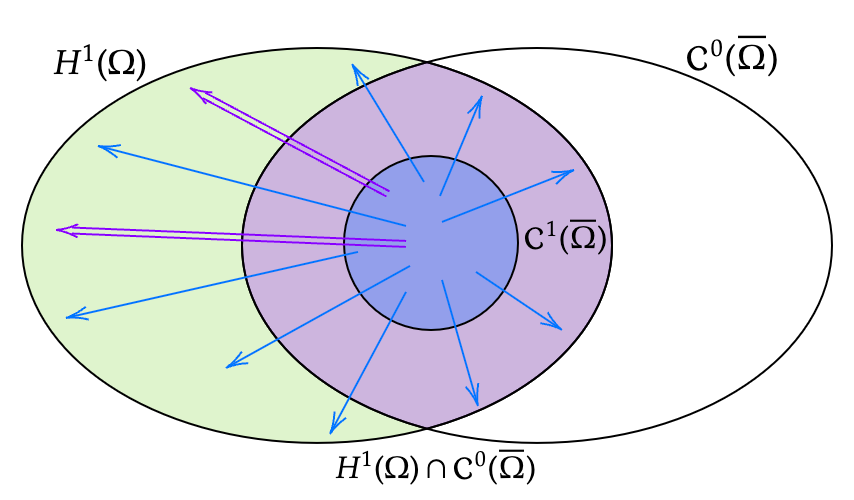
\includegraphics[width=0.9\linewidth]{images/density}\ \ }
\end{Figure}

Before doing so, we need the following: assume $\partial\Omega\in\Cc^\infty$, for every $x_0\in\partial\Omega$ we define $H^s(U_{x_0})$ where $U_{x_0}\subset\RR^{n-1}$ in the sense of local charts, so we found the meaning of $H^s(\partial\Omega)$.

\rule{0.31\textwidth}{0.2pt}
\smallskip

\textbf{Thm.} Let $\Omega\subset\RR^n$ open bdd with $\Cc^\infty$ boundary, and $k\in\NN$. Then, $\exists\,!$ lin. cont. surj. operator 
\begin{gather*}
\gamma_{_0}:H^1(\Omega)\to H^{1/2}(\partial\Omega)\quad\text{such that} \\
\gamma_{_0} u=u\big|_{\partial\Omega}\quad\forall\, u\in\Cc^0(\overline{\Omega})\big(\cap H^1(\Omega)\text{ obv}\big)
\end{gather*}
Moreover, $\exists$ lin. cont. operator 
\begin{gather*}
\Rc:H^{1/2}(\partial\Omega)\to H^1(\Omega)\quad\text{such that} \\
\gamma_{_0}(\Rc g)=g\qquad\forall\, g\in H^{1/2}(\partial\Omega)
\end{gather*}

We call $\gamma_{_0}$ \textbf{trace operator} of order 0, and $\Rc$ \textbf{lift operator} (rilevamento).

\smallskip

\textbf{Rmk:} $\gamma_{_0}$ is unique thanks to the density prop. stated before, $\Rc$ is not unique cause $\gamma_{_0}$ not inv.

\rule{0.31\textwidth}{0.2pt}
\smallskip

\textbf{Thm.} Let $\Omega\subset\RR^n$ open bdd with $\Cc^\infty$ boundary, and $k\in\NN$. Then, $\exists\,!$ $k$ lin. cont. surj. operators $\gamma_{_0},\dots,\gamma_{k-1}$ defined as
\begin{gather*}
\gamma_j:H^k(\Omega)\to H^{k-j-1/2}(\partial\Omega)\quad\forall\,j=0:k-1\\
\text{s.t.}\qquad
\gamma_j u=\frac{\partial^j u}{\partial\nu^j} \bigg|_{\partial\Omega}\qquad\forall\, u\in \Cc^0(\overline{\Omega})
\end{gather*}

We call $\gamma_j$ \textbf{trace operator} of order $j$.

\rule{0.31\textwidth}{0.2pt}
\smallskip

Finally, we can give a characterization of $H^k_0$:

\smallskip

\textbf{Thm.} Let $\Omega\subset\RR^n$ open bdd with $\Cc^\infty$ boundary, $u\in H^k(\Omega)$, with $k\in\NN$. Then:
\begin{equation*}
u\in H^k_0(\Omega) \quad\Longleftrightarrow\quad \gamma_j=0\quad\forall\,j=0:k-1
\end{equation*}

In other words: $H^k_0(\Omega)=\bigcup_j\text{ker}_{\gamma_j}\,.$

\rule{0.31\textwidth}{0.2pt}

% =================================================

\subsection{\texorpdfstring{\color{red}Embedding Thms in \texorpdfstring{$H^k,\ k\in\NN,$}{C} in dim. \texorpdfstring{$n\geq 2$}{C}}{}}

% =================================================

\textbf{Thm (Sobolev).} $\Omega\subset \RR^n$ open with $\partial\Omega\in\text{Lip}$ (or $\Omega=\RR^n$). Then:
\begin{align*}
n=2k\ \leadsto\ &H^k(\Omega)\subset L^p(\Omega)\quad \forall p\in [2,\infty) \\
n>2k\ \leadsto\ &H^k(\Omega)\subset L^p(\Omega)\quad \forall p\in [2,2^*] \\
\begin{array}{c}
\exists\, m\in\NN\text{ s.t.}\\
n<2(k-m)   
\end{array}& 
\leadsto\ H^k(\Omega)\subset \Cc^m(\overline{\Omega})\cap L^\infty(\Omega)\qquad
\end{align*}
where $2^*=\nicefrac{2n}{n-2k}$ is the critical exponent.

\smallskip

\textbf{Rmk:} also for $H^k_0$ without assumptions on $\partial\Omega$.

\rule{0.31\textwidth}{0.2pt}
\smallskip

\textbf{Thm (Sobolev, Rellich, Gagliardo, Nirenberg).} $\Omega\subset \RR^n$ bdd open with $\partial\Omega\in\text{Lip}$.
\begin{align*}
n=2k\ \leadsto\ &H^k(\Omega)\subset\subset L^p(\Omega)\quad \forall p\in [1,\infty) \\
n\geq 2k\ \leadsto\ &H^k(\Omega)\subset\subset L^p(\Omega)\quad \forall p\in [1,2^*)
\end{align*}

\smallskip

\textbf{Rmk:} $p=1$ thx to $L^p$-spaces inclusion ($\Omega$ bdd).

\rule{0.31\textwidth}{0.2pt}

% =================================================

\subsection{\texorpdfstring{\color{red}The spaces \texorpdfstring{$H^{-k},\ k\in\NN,$}{C} in dim. \texorpdfstring{$n\geq 2$}{C}}{}}

% =================================================

$H^{-s}(\Omega):=\left[ H^s_0(\Omega) \right]'$, $H^{-s}(\partial\Omega):=\left[ H^s(\partial\Omega) \right]'$

\rule{0.31\textwidth}{0.2pt}
\smallskip

Let $u:\Omega\subset\RR^n\to\RR^n$.

\smallskip

\textbf{Def.} $\mathbf{E}(\Omega)=\left\{ u\in \mathbf{L}^2(\Omega);\, \nabla\!\!\cdot\! u \in L^2(\Omega) \right\}\equiv \mathbf{L}^2_{\text{div}}$ in the sense of distributions, i.e.
\begin{equation*}
\int_\Omega u\cdot \nabla\varphi=-\int_\Omega (\nabla\cdot u)\, \varphi\quad\forall\,\varphi\in\Dc(\Omega)
\end{equation*}

\smallskip

\textbf{Rmk:} if $n=1$ then $H^1(\Omega)\equiv E(\Omega)$.

\rule{0.31\textwidth}{0.2pt}
\smallskip

\textbf{Thm.} Let $\Omega\subset\RR^n$ open bdd with $\partial\Omega\in\Lip$. Then, $\exists\,!$ lin. cont. surj. operator 
\begin{gather*}
\gamma_{_\nu}:\Ev(\Omega)\to H^{\text{-}1/2}(\partial\Omega)\quad\text{such that} \\
\gamma_{_\nu} u=u\cdot\nu\qquad\forall\, u\in\left[\Cc^0(\overline{\Omega})\right]^n
\end{gather*}

We call $\gamma_{_\nu}$ \textbf{normal trace operator}.

\rule{0.31\textwidth}{0.2pt}
\smallskip

\textbf{Thm (Generalized Gauss-Green formula).} Let $\Omega\subset\RR^n$ open bdd with $\partial\Omega\in\Lip$. Then:
\begin{equation*}
\int_\Omega\!\! u\cdot\nabla\varphi+\int_\Omega\!\varphi\,\Div u={}_{_{H^{\nicefrac{\text{-}1}{2}}}}\!\!\sca{\gamma_{_\nu} u,\,\gamma_{_0}\varphi}\!\!{}_{_{H^{\nicefrac{1}{2}}}}
\end{equation*}

$\forall\, u\in\Ev(\Omega),\ \varphi\in H^1(\Omega)$.

\rule{0.31\textwidth}{0.2pt}
\smallskip

We'll apply this to $u:\Omega\to\RR$ (e.g. Neumann problem) where $u\in H^1$ with $\Delta u\in L^2$. Indeed, $\nabla u \in \mathbf{L^2}$ with $\nabla\!\cdot\!\nabla u \in L^2$, i.e. $\nabla u \in \mathbf{E}$. Then $\exists\, !$
\begin{equation*}
\gamma_{_\nu} \nabla u=\nabla u \cdot \nu = \frac{\partial u}{\partial \nu} 
\end{equation*}
and the Gauss-Green formula becomes
\begin{equation*}
\int_\Omega\!- \Delta u\ v=\int_\Omega \nabla\! u\,\nabla\! v -\sca{\frac{\partial u}{\partial \nu}, \gamma_{_0} v}\quad\forall\, v\in H^1
\end{equation*}

\rule{0.31\textwidth}{1pt}











%!TEX root = ../main.tex

% =================================================
% =================================================

\vspace{-1em}

\section{\texorpdfstring{\color{forestgreen(web)}Exercise Classes Stuff}{}}

% =================================================
% =================================================

E.g. Sobolev ineq., Regularity theory, etc.

\rule{0.31\textwidth}{1pt}

\newpage

%!TEX root = ../main.tex

% =================================================
\textbf{Recalls on integration.}
\begin{align*}
&\int_a^b f'g\dx = \big[ fg \big]_a^b-\int_a^b fg'\dx \\
&\int_\Omega \nabladot\fv\ g=\int_{\partial\Omega}\fv\!\cdot\!\nu\ g-\int_\Omega \fv\ \nabla g \\
&\int_\Omega \underbracket[0.5pt]{\nabladot\left(\nabla u\right)}_{\Delta u}\,v=\int_{\partial\Omega}\underbracket[0.5pt]{\nabla u\!\cdot\!\nu\,}_{\nicefrac{\partial u}{\partial \nu}}\,v-\int_\Omega \nabla u\,\nabla v
\end{align*}

\rule{0.31\textwidth}{0.2pt}

% =================================================
\textbf{Recalls on weak derivatives.}
\begin{align*}
&\int_\Omega \dfrac{\partial u}{\partial x_i}\,\varphi = \int_\Omega u\,\dfrac{\partial\varphi}{\partial x_i} \\ 
&\int_\Omega (\nabladot \uv)\,\varphi = -\int_\Omega \uv\cdot\nabla\varphi \\
&\int_\Omega \Delta \uv\ \varphi = -\int_\Omega \nabla\uv\cdot\nabla\varphi
\end{align*}

\rule{0.31\textwidth}{1pt}

% =================================================
% =================================================

\vspace{-1em}

\section{\texorpdfstring{\color{forestgreen(web)}Linear PDEs}{}}

% =================================================
% =================================================

$n\geq 2$, $\Omega\subset\RR^n$ open bdd with \emph{smooth} boundary

% =================================================

\subsection{\texorpdfstring{\color{red}Homogeneous Dirichlet problem}{}}

% =================================================

$\alpha\in\RR$, find $u:\Omega\to\RR$ st
\begin{equation*}
\begin{cases}
    -\Delta u +\alpha u = f &\text{ in }\Omega\\
    u=0 &\text{ on }\partial\Omega    
\end{cases}
\end{equation*}

\textbf{Def (Classical sol).} $u\in\Cc^2(\Omega)\cap\Cc^0(\overline{\Omega})$

\smallskip

\textbf{Rmk:} $u$ classical sol $\Rightarrow$ $f\in\Cc^0(\Omega)$, conversely, $f\notin\Cc^0(\Omega)$ $\Rightarrow$ $u$ cannot be classical sol.

\rule{0.31\textwidth}{0.2pt}
\smallskip

\textbf{Def (Weak sol).} $u\in H^1_0(\Omega)$ such that
\begin{equation*}
\int_{_\Omega}\!\!\!  \nabla u\,\nabla v +\alpha\!\!\int_{_\Omega}\!\!\!  uv ={}_{_{H^{\text{-}1}}}\!\!\sca{f,v}{}_{_{\!\!H^1_0}}\quad\forall\, v\in H^1_0(\Omega)
\end{equation*}

\rule{0.31\textwidth}{0.2pt}
\smallskip

Since $u\in H^1_0(\Omega)$ $\Leftrightarrow$ $u\big|_{\partial \Omega}=0$, classical $\Rightarrow$ weak, and weak + reg. $\Rightarrow$ classical

\rule{0.31\textwidth}{0.2pt}
\smallskip

\textbf{Thm.} Let $\alpha\geq 0$, $f\in H^{\text{-}1}(\Omega)$. Then $\exists\,!$ weak sol $u\in H^1_0(\Omega)$. Moreover, there holds the \textbf{Dirichlet principle}, i.e. $u$ unique minimizer over $H^1_0\Omega)$ of 
\begin{equation*}
J(w)=\frac{1}{2}\int_{_\Omega}\!\!\!  \Big( \left| \nabla w \right|^2+\alpha\left| w \right|^2 \Big)-\sca{f,w}
\end{equation*}

\textbf{Rmk:} the least eigenvalue is 
\begin{equation*}
0<\lambda_1:=\inf_{H^1_0\setminus\{0\}} \frac{\norm{\nabla u}_2^2}{\norm{u}_2^2}=\frac{1}{C_\Omega^2}  
\end{equation*}

thus coercivity still holds for $\alpha>-\lambda_1$. For $\alpha\leq -\lambda_1$ we apply Fredholm's alternative (but no more Dirichlet principle) thx to $H^1\subset\subset L^2$.

\rule{0.31\textwidth}{0.2pt}

% =================================================

\subsection{\texorpdfstring{\color{red}Inhomogeneous Dirichlet problem}{}}

% =================================================

$\alpha\in\RR$, find $u:\Omega\to\RR$ st
\begin{equation*}
\begin{cases}
    -\Delta u +\alpha u = f &\text{ in }\Omega\\
    u=g &\text{ on }\partial\Omega    
\end{cases}
\end{equation*}

\textbf{Def (Classical sol).} $u\in\Cc^2(\Omega)\cap\Cc^0(\overline{\Omega})$

\smallskip

\textbf{Rmk:} $u$ classical sol $\Rightarrow$ $f\in\Cc^0(\Omega)$, $g\in\Cc^0(\partial\Omega)$

\rule{0.31\textwidth}{0.2pt}
\smallskip

$K:=\left\{ v\in H^1(\Omega);\ \gamma_{_0}v=g \right\}\equiv H^1_g(\Omega)$

\smallskip

\textbf{Def (Weak sol).} $u\in K$ such that
\begin{equation*}
\int_{_\Omega}\!\!\! \nabla u\,\nabla v +\alpha\!\!\int_{_\Omega}\!\!\! uv ={}_{_{\left[H^1\right]'}}\!\sca{f,v}{\!}_{_{H^1_0}}\quad\forall\, v\in H^1_0(\Omega)
\end{equation*}

\rule{0.31\textwidth}{0.2pt}
\smallskip

classical $\Rightarrow$ weak, and weak + reg. $\Rightarrow$ classical

\rule{0.31\textwidth}{0.2pt}
\smallskip

\textbf{Thm.} Let $\alpha> -\lambda_1$, $f\in\left[ H^1(\Omega) \right]'$, $g\in H^{1/2}(\partial\Omega)$. Then $\exists\,!$ weak sol $u\in K$. Moreover, $u$ is the unique minimizer over $K$ of 
\begin{equation*}
J(w)=\frac{1}{2}\int_{_\Omega}\!\!\!  \Big( \left| \nabla w \right|^2+\alpha w^2 \Big)-\sca{f,w}
\end{equation*}

\textbf{\color{lavender(floral)}Proof.} See whiteboards u.u

\rule{0.31\textwidth}{0.2pt}

% =================================================

\subsection{\texorpdfstring{\color{red}Inhomogeneous Neumann problem}{}}

% =================================================

$\alpha>0$, $f\in L^2(\Omega)$, $g\in H^{\text{-}1/2}(\partial\Omega)$,
\begin{equation*}
\begin{cases}
    -\Delta u +\alpha u = f &\text{ in }\Omega\\
    \dfrac{\partial u}{\partial\nu}=g &\text{ on }\partial\Omega    
\end{cases}
\end{equation*}

\textbf{Def (Classical sol).} $u\in\Cc^2(\Omega)\cap\Cc^1(\overline{\Omega})$

\smallskip

\textbf{Rmk:} $u$ classical sol $\Rightarrow$ $f\in\Cc^0(\Omega)$, $g\in\Cc^0(\partial\Omega)$

\rule{0.31\textwidth}{0.2pt}
\smallskip

\textbf{Def (Weak sol).} $u\in H^1(\Omega)$ such that
\begin{equation*}
\int_{_\Omega}\!\!\! \nabla u\,\nabla v +\alpha\!\!\int_{_\Omega}\!\!\! uv =\int_{_\Omega}\!\!\!fv+\sca{g,\gamma_{_0}v}\quad\forall\, v\in H^1
\end{equation*}

where $\sca{\cdot,\cdot}$ is between $H^{\text{-}1/2}$ and $H^{1/2}$.

\smallskip

\textbf{Rmk:} the weak form. is obtained by using the generalized GG formula, since $\nabla u \in \mathbf{E}$.

\rule{0.31\textwidth}{0.2pt}
\smallskip

classical $\Rightarrow$ weak, and weak + reg. $\Rightarrow$ classical

\rule{0.31\textwidth}{0.2pt}
\smallskip

\textbf{Thm.} Let $\alpha>0$ (least eigenv.), $f\in L^2(\Omega)$, $g\in H^{\text{-}1/2}(\partial\Omega)$. Then $\exists\,!$ weak sol $u\in H^1(\Omega)$. Moreover, $u$ is the unique minimizer over $H^1$ of 
\begin{equation*}
J(w)=\frac{1}{2}\int_{_\Omega}\!\!\!  \Big( \left| \nabla w \right|^2+\alpha w^2 \Big)-\int_\Omega\!\!\!fw-\sca{g,\gamma_{_0}w}
\end{equation*}


\rule{0.31\textwidth}{0.2pt}

% =================================================

\subsection{\texorpdfstring{\color{red}Helmholtz-Weyl scomposition}{}}

% =================================================

Check FSI

\rule{0.31\textwidth}{0.2pt}

% =================================================

\subsection{\texorpdfstring{\color{red}Stokes problem (stationary NS linearized)}{}}

% =================================================
 
Check FSI

\rule{0.31\textwidth}{1pt}





%!TEX root = ../main.tex

% =================================================
% =================================================

\vspace{-1em}

\section{\texorpdfstring{\color{forestgreen(web)}Nonlinear PDEs}{}}

% =================================================
% =================================================

$n\geq 2$, $\Omega\subset\RR^n$ open bdd with \emph{smooth} boundary

% =================================================

\subsection{\texorpdfstring{\color{red}Homogeneous Dirichlet problem (semilinear)}{}}

% =================================================

$f:\RR\to\RR$, $f\in\Cc^1(\RR)$,
\begin{equation*}
\begin{cases}
    -\Delta u = f(u) &\text{ in }\Omega\\
    u=0 &\text{ on }\partial\Omega    
\end{cases}
\end{equation*}

\rule{0.31\textwidth}{0.2pt}
\smallskip

\textbf{Brezis-Kato condition.} $n\geq 3$, $f$ satisfies the BK condition if $\exists\, C>0$ s.t.
\begin{equation*}
\left| f(s) \right|\leq C\left( 1+|s|^{2^*-1} \right)\qquad \forall\, s\in\RR \tag{BK}
\end{equation*}

where $2^*=\nicefrac{2n}{n-2}$ is the critical Sobolev exp. 

\smallskip

\textbf{Rmk:} $n\geq 3$ because for $n=2$ there is no critical exp, but one can write the BK cond. as
\begin{equation*}
\exists\, C\!>\!0,\,\overline{p}\!\in\![2,\infty)\, :\, \left| f(s) \right|\!\leq\! C\!\left( 1+|s|^{\overline{p}} \right)\ \forall\, s\!\in\!\RR
\end{equation*} 

\vspace{-1em}

\rule{0.31\textwidth}{0.2pt}
\smallskip

\textbf{Def (Weak sol).} If BK holds, we can say that $u\in H^1_0(\Omega)$ is a weak solution if
\begin{equation*}
\int_\Omega \nabla u\ \nabla v=\int_\Omega f(u)\ v\quad\forall\,v\in H^1_0(\Omega)
\end{equation*}

\rule{0.31\textwidth}{0.2pt}
\smallskip

\textbf{Thm (Brezis-Kato).} $n\geq 3$, if BK holds then every weak sol is a classical sol.

\smallskip

\textbf{\color{lavender(floral)}Proof.} See whiteboards u.u

\rule{0.31\textwidth}{0.2pt}

% =================================================

\subsection{\texorpdfstring{\color{red}The role of the critical Sobolev exponent}{}}

% =================================================

\textbf{Def.} $X$ Banach, $J:X\to\RR$ functional. We say that $J$ is continuous if
\begin{equation*}
u_m\xrightarrow{X} u\quad \Longrightarrow\quad J(u_m)\rightarrow J(u)
\end{equation*}

In addiction, we say that $J$ if Fréchet differentiable at $u$ if $\exists\,L\in X'$ s.t.
\begin{equation*}
\lim_{\norm{u_m-u}\to 0}\frac{J(u_m)-J(u)-\sca{L,u_m-u}}{\norm{u_m-u}} =0
\end{equation*}

and we put $L=J'(u)$.

\rule{0.31\textwidth}{0.2pt}
\smallskip

$X=H^1_0(\Omega)$, $J(u)=\norm{\nabla u}_2^2$, then
\begin{equation*}
\sca{J'(u),v}=2\int_\Omega \nabla u\ \nabla v
\end{equation*}

$X=L^p(\Omega)$, $2\leq p <\infty$, $J(u)=\norm{\nabla u}_p^p$, then
\begin{equation*}
\sca{J'(u),v}=p\int_\Omega |u|^{p-2}\,u\,v
\end{equation*}

\rule{0.31\textwidth}{0.2pt}
\smallskip

\textbf{Thm.} $n\geq 3$, if $2< p < 2^*$ then
\begin{equation*}
\circledast\,
\begin{cases}
    -\Delta u = u^{p-1} &\text{ in }\Omega\\
    u >0 &\text{ in }\Omega\\
    u=0 &\text{ on }\partial\Omega    
\end{cases}
\end{equation*}
admits at least one solution.

\smallskip

\textbf{\color{lavender(floral)}Proof.} See whiteboards u.u

\rule{0.31\textwidth}{0.2pt}
\smallskip

\textbf{Def.} $n\geq 2$, $\Omega\subset\RR^n$ is starshaped wrt $y\in\Omega$ if $\forall\, x \in\Omega$ the segment $xy$ is contained in $\Omega$.

\rule{0.31\textwidth}{0.2pt}
\smallskip

\textbf{Thm (Pohozaev).} $n\geq 3$, $\Omega\subset\RR^n$ bounded starshaped domain, $p\geq 2^*$. Then $\circledast$ admits no classical sol (even with $u\neq 0$ in $\Omega$).

\rule{0.31\textwidth}{0.2pt}
\smallskip

\textbf{Thm (Ni-Servin).} $n\geq 3$, the problem
\begin{equation*}
\begin{cases}
    -\Delta u = u^{p-1} &\text{ in }\RR^n\\
    u \geq 0 &\text{ in }\RR^n  
\end{cases}
\end{equation*}

admits only $u\equiv 0$ as solution for $2<p<2^*$, instead $\exists\,\infty$-many solution for $p\geq 2^*$.

\rule{0.31\textwidth}{0.2pt}

% =================================================

\subsection{\texorpdfstring{\color{red}Stationary NS problem (quasilinear)}{}}

% =================================================

Check FSI

\rule{0.31\textwidth}{1pt}











%!TEX root = ../main.tex

% =================================================
% =================================================

\vspace{-1em}

\section{\texorpdfstring{\color{forestgreen(web)}Evolution Problems}{}}

% =================================================
% =================================================

% =================================================

\subsection{\texorpdfstring{\color{red}Bochner Integral}{}}

% =================================================
 
Check FSI

\rule{0.31\textwidth}{0.2pt}

% =================================================

\subsection{\texorpdfstring{\color{red}Heat Equation}{}}

% =================================================

Check FSI

\rule{0.31\textwidth}{0.2pt}

% =================================================

\subsection{\texorpdfstring{\color{red}Wave Equation}{}}

% =================================================

Check FSI

\rule{0.31\textwidth}{0.2pt}

% =================================================

\subsection{\texorpdfstring{\color{red}Evolution NS Equation}{}}

% =================================================

Check FSI

\rule{0.31\textwidth}{1pt}

% =================================================
% =================================================

\vspace{-1em}

\section{\texorpdfstring{\color{forestgreen(web)}Conservation Laws}{}}

% =================================================
% =================================================

Missing

\rule{0.31\textwidth}{0.2pt}

% =================================================

\subsection{\texorpdfstring{\color{red}Korteweg - de Vries}{}}

% =================================================

Missing

\rule{0.31\textwidth}{1pt}


\end{multicols*}

\newpage

\setcounter{equation}{0}

\chapter*{Fluid-Structure Interaction}

\begin{center}
Let $n\geq 2$, $\Omega\subset\RR^n$ open bdd with \emph{smooth} boundary (except in specified cases). 
\end{center}

\begin{multicols*}{2}

\setlength{\columnseprule}{1pt}
\def\columnseprulecolor{\color{teal}}

%!TEX root = ../main.tex

% =================================================
% =================================================

\FSIsection{Helmholtz-Weyl scomposition}

% =================================================
% =================================================

We consider vectorial fields $\bm{u}:\Omega\subseteq\RR^n\to\RR^n$. Capital bold letters denote vectorial functional spaces, e.g. $\mathbf{L}^2(\Omega)=\left[ L^2(\Omega) \right]^n$ or $\mathbf{H}^1(\Omega)= \left[ H^1(\Omega) \right]^n$.

\smallskip

Let $\Omega$ be omitted. We can exploit what we already know, such as
\begin{itemize}

\item[$\triangleright$] $\Lv^2$ is Hilbert with $\norm{\bm{u}}_{\Lv^2}^2=\displaystyle\int_\Omega \abs{\bm{u}}^2=\sum_{i=1}^n \norm{u_i}^2_{L^2}$

\item[$\triangleright$] $\Hv^1$ is Hilbert with
\begin{equation*}
(\bm{u},\bm{v})_{\Hv^1}=(\bm{u},\bm{v})_{\Lv^2}+(\nabla\bm u,\nabla \bm v)_{\Lv^2}= \int_\Omega \Big( \nabla\bm u : \nabla \bm v + \bm u \bm v \Big)
\end{equation*}
where $\nabla\bm u:\nabla\bm v$ stands for the \emph{Euclidean scalar product} of the Jacobian matrices of $\bm u$ and $\bm v$. 

\item[$\triangleright$] $\Hv_0^1\coloneq\overline{\bm \Dc}^{\,\Hv^1}\!$ is Hilbert, and via \emph{Poincaré's inequality}
\begin{equation*}
(\bm u,\bm v)_{\Hv^1}\approx(\bm u,\bm v)_{\Hv^1_0}=(\nabla\bm u,\nabla \bm v)_{\Lv^2}=\int_\Omega \nabla\bm u : \nabla \bm v
\end{equation*}
where symbol $\approx$ denotes \emph{equivalent norms}.

\item[$\triangleright$] $\Ev\coloneq \left\{ \bm u\in \mathbf{L}^2;\ \nabla \cdot \bm u \in L^2 \right\}\equiv \Lv^2_{\text{div}}$ is Hilbert with
\begin{equation*}
(\bm u,\bm v)_\Ev=(\bm u,\bm v)_{\Lv^2}+(\nabla \cdot \bm u,\nabla \cdot\bm v)_{L^2} 
\end{equation*}

Since $\nabla\bm u\in \Lv^2 \impliesnotimplied \nabla\cdot\bm u\in L^2$ (only if $n=1$), then $\Hv^1 \subsetneqq \Ev \subset \Lv^2$. 

We remark that when we say $\nabla\cdot\bm u\in L^2$ we mean in weak (distributional) sense. Indeed, given $\bm u\in\Lv^2$ its weak divergence $\nabla\cdot \bm u\in H^{-1}$ is well defined as
\begin{equation*}
\dualH{\nabla\cdot\bm u,\ \varphi}{-1}{1}{0}=-\int_\Omega \bm u\cdot \nabla \varphi\qquad \forall\, \varphi \in H^1_0\ (\in\Dc)
\end{equation*}

If it happens that $\nabla\cdot \bm u$ is not only $H^{\text{-}1}\!$ but also $L^2$, then $\bm u\in \Ev$ \\ (\emph{"$\bm u$ in $\Lv^2$ with weak divergence in $L^2$, then $\bm u$ in $\Ev$" sounds similar to the older "$u$ in $L^2$ with weak derivative $u'$ in $L^2$, then $u$ in $H^1$"}).

Moreover, for $\bm u\in\Ev$ the normal component of its trace $\gamma_{_\nu}(\bm u)\in H^{\text{-}1/2}$ is well defined and satisfy the \textbf{Generalized Gass-Green formula} (even if $\Omega$ is only Lipschitz):
\begin{equation}
\label{eq:GG}
\int_\Omega \bm u\cdot \nabla \varphi+\int_\Omega \big(\nabla\cdot\bm u\big)\, \varphi = \dualT{\gamma_{_\nu}\bm u,\ \gamma_{_0}\varphi}{-1/2}{1/2}\qquad \forall \,\varphi\in H^1
\end{equation}

Hence, in some way $\Ev$ is an intermediate space: in $\Lv^2$ there are no traces, in $\Ev$ only normal traces, in $\Hv^1$ full traces. One can go through the def. of $\Lv^2_{\text{curl}}$ to find out that there only tangent traces are defined and, via \emph{Friedrich's inequality}, $\Lv^2_{\text{div}}\oplus\Lv^2_{\text{curl}}=\Hv^1$.

\end{itemize}

Let us introduce the following new spaces:
\begin{itemize}
\item[$\triangleright$] $\bm\Vc \coloneq \left\{ \bm u\in\bm\Dc;\ \nabla\cdot\bm u=0 \text{ in }\Omega \right\}$

\item[$\triangleright$] $\Vv\coloneq \overline{\bm\Vc}^{\Hv^1} \!= \left\{ \bm u\in\mathbf{H}_0^1;\ \nabla\cdot\bm u=0\text{ in }\Omega\right\}\equiv\Hv^1_{0,\sigma}$, which is a closed subspace of $\Hv^1_0$ and hence, it is Hilbert if endowed with
\begin{equation*}
(\bm u,\bm v)_\Vv=(\nabla \bm u,\nabla \bm v)_{\Lv^2} 
\end{equation*}

Obviously, $\Vv\subset\Ev$ since free-div. $\impliesnotimplied$ $L^2$-div.

\item[$\triangleright$] $\Gv_1\coloneq \overline{\bm\Vc}^{\Lv^2} \!= \left\{ \bm u\in\mathbf{L}^2;\ \nabla\cdot\bm u=0,\ \gamma_{_\nu} \bm u=0 \right\}\subset\Ev$ 

$\mathbf{G}_2=\left\{ \bm u\in\mathbf{L}^2;\ \nabla\cdot\bm u=0,\ \exists\,g\in H^1\text{ s.t. }\bm u=\nabla g \right\}\subset\Ev$ 

$\mathbf{G}_3=\left\{\bm u\in\mathbf{L}^2;\ \exists\,g\in H^1_0\text{ s.t. }\bm u=\nabla g \right\}\centernot\subset\Ev$

We remark that in $\Gv_2$, the incompressibility constraint makes the scalar function $g$ harmonic:
\begin{equation*}
0=\nabla\cdot\bm u=\nabla\cdot\nabla g=\nabla^2 g=\Delta g
\end{equation*}
Instead, if you add the constraint in $\Gv_3$, you obtain $g\equiv 0$.

\item[$\triangleright$] $\Ev_0\coloneq \ker(\gamma_{_\nu})=\left\{ \bm u\in\Ev;\ \gamma_{_\nu} \bm u=0 \right\}\subset \Ev $
\end{itemize}
\vspace{-0.5em}
\rule{0.495\textwidth}{0.2pt}\smallskip

All these definitions lead to the following properties:
\vspace{-0.5em}
\begin{gather*}
\bm\Vc \overset{\delta}{\subset} \Vv \overset{\delta}{\subset} \Gv_1\subset\Ev_0, \qquad \Gv_1\oplus\Gv_2\subset\Ev, \qquad \Gv_2\cap \Ev_0=\{\bm 0\},\\
\Gv_3 \cap \Ev = \left\{ \bm u \in \Lv^2;\ \exists\,g\in H^2\cap H^1_0 \text{ s.t. }\bm u=\nabla g \right\}, \\
\Gv_3 \cap \Ev_0 = \left\{ \bm u \in \Lv^2;\ \exists\,g\in H^2_0 \text{ s.t. }\bm u=\nabla g \right\}.
\end{gather*}

\textbf{\color{lavender(floral)}Proof.} See whiteboard \texttt{FSI-1} u.u

\smallskip

Instead, in dimension $n=1$ there hold
\begin{gather*}
\Ev\equiv H^1,\quad \bm\Vc=\{0\}\ \Longrightarrow\ \Vv=\Gv_1=\{0\},\\ \Gv_2=\RR,\quad \Gv_3=\big\{ u\in L^2;\ \underbracket[0.5pt]{\textstyle\int_\Omega u=0}_{\scriptstyle\text{zero average}}\big\}\equiv L^2_0.
\end{gather*}

\vspace{-0.5em}
\rule{0.495\textwidth}{0.2pt}\smallskip

\textbf{Thm(H-W scomposition).} $\Gv_1,\ \Gv_2,\ \Gv_3$ are mutually orthogonal (w.r.t. the $\Lv^2$ scalar product), and $\mathbf{L}^2=\mathbf{G}_{1}\oplus\mathbf{G}_{2}\oplus\mathbf{G}_{3}$. In other \emph{words}: 
\begin{gather*}
\mathbf{G}_{i}\perp\mathbf{G}_{j}\ \ \forall\,i\neq j,\qquad \forall\, \bm f \in \Lv^2\ \exists!\,(\bm f_1,\bm f_2,\bm f_3)\in\Gv_1\!\times\!\Gv_2\!\times\!\Gv_3 \\
\qquad\qquad\qquad\qquad\text{ s.t. }\bm f= \bm f_1+\bm f_2+\bm f_3.
\end{gather*}

\textbf{\color{lavender(floral)}Proof.} See whiteboard \texttt{FSI-2} u.u 

\noindent\rlap{\rule[1.5ex]{0.495\textwidth}{.2pt}}
%\rule{0.495\textwidth}{0.2pt}

\newcolumn

% =================================================
% =================================================

\FSIsection{Stokes Problem (Stationary Linearized NS)}

% =================================================
% =================================================

Let us consider the following problem:
\begin{subequations}
    \label{Stokes-problem}
    \begin{align}[left=\empheqlbrace]
    -\eta\Delta \bm u +\nabla p = \bm f &\qquad\text{ in }\Omega  \label{eq:sp1} \\
    \nabla\cdot \bm u=0 &\qquad\text{ in }\Omega \label{eq:sp2} \\
    \bm u=0 &\qquad\text{ on }\partial\Omega \label{eq:sp3}
    \end{align}
\end{subequations}

where $\bm u=(u_1,\dots,u_n)$ (you may think $n=3$) is the velocity vector, $\Delta\bm u$ is the vector laplacian, $p$ is the scalar pressure of the fluid, $\eta>0$ its dynamic viscosity, and $\bm f\in\mathbf{L}^2$ is a given vector function representing the density of the external force applied to the fluid.

Condition \eqref{eq:sp2} represents the \emph{incompressibility constraint}, while \eqref{eq:sp3} the \emph{non-slip boundary condition}, i.e. the case in which the fluid is adherent to the boundary of $\Omega$. One can use different bcs as long as there holds the GG formula \eqref{eq:GG} for $\bm u$ and $1$, which acts as a compatibility condition:
\begin{equation*}
\int_\Omega \bm u\ \cancel{\nabla 1} + \int_\Omega \big(\cancel{\nabla\cdot \bm u}\big)\, 1= \sca{\gamma_{_\nu}\bm u, 1}\quad\leadsto\quad \sca{\gamma_{_\nu}\bm u, 1}=0
\end{equation*}

In system \eqref{Stokes-problem}, the unknowns we look for are $\bm u$ and $p$. Notiche that \eqref{eq:sp1}+\eqref{eq:sp2} are $n+1$ scalar equations in the $n+1$ unknowns $u_1,\dots,u_n,p$ while \eqref{eq:sp3} gives just $n$ bcs. The reason is that $p$ appears in $\eqref{eq:sp1}$ only through its gradient, therefore the pressure is determined up to an additive constant (if $\overline{p}$ is a solution, $\overline{p}+k$ is a solution too). 

\noindent\rlap{\rule[1.5ex]{0.495\textwidth}{.2pt}}

\vspace{-0.5em}

\FSIsubsection{Variational Formulation}

It is natural to think about $\bm u\in\Vv$ and $p\in H^1\!/\RR$, then \eqref{eq:sp1} becomes
\begin{equation*}
\int_\Omega -\eta\Delta\bm u\ \bm v +\int_\Omega \nabla p\ \bm v =\int_\Omega \bm f\ \bm v\qquad \forall\, \bm v\in\Vv
\end{equation*}

The integrations by parts yield
\begin{equation*}
\eta \int_\Omega \nabla\bm u:\nabla\bm v-\int_{\partial\Omega}\eta\,\frac{\partial \bm u}{\partial \nu}\ \cancel{\bm v}+\int_{\partial\Omega} \cancel{\bm v} \cdot \nu\ p -\int_\Omega \cancel{\nabla\cdot\bm v}\ p = \int_\Omega \bm f\ \bm v
\end{equation*}

Then the \textbf{weak formulation} is 
\begin{equation*}
\big(\forall\,\bm f\in\Lv^2\big)\text{ Find }\bm u\in \Vv\text{ :}\quad \eta\int_\Omega \nabla \bm u : \nabla \bm v=\int_\Omega \bm f\ \bm v\quad \forall\,\bm v\in\mathbf{V}\tag{WF1}
\end{equation*}

By LM (\textbf{\color{lavender(floral)}Proof:} See wb \texttt{FSI-3} u.u), $\big(\forall\,\bm f\in\Lv^2\big)$ $\exists\,!\,\bm u \in \mathbf{V}$ satisfying (WF1).

\noindent\rlap{\rule[1.5ex]{0.495\textwidth}{.2pt}}\vspace{-0.5em}

Now we are at the lowest level, but we'd like to recover the pressure in the formulation. Applying the blackbox called \emph{elliptic regularity theory}, 
\begin{equation*}
\big(\forall\,\bm f\in\Lv^2\big)\ \exists\,!\,\bm u \in \mathbf{V}\cap\Hv^2 \textit{ satisfying }\text{(WF1)}
\end{equation*}

Then undo the int. by parts over $\Delta\bm u$, and since $\Vv$ is dense in $\Gv_1$:
\begin{equation*}
\big(\forall\,\bm f\in\Lv^2\big)\ \exists\,!\,\bm u \in \mathbf{V}\cap\Hv^2 \textit{ satisfying } \int_\Omega \Big( \eta\Delta \bm u+\bm f\Big)\bm v=0\ \ \forall\,\bm v\in\Gv_1
\end{equation*}

This means that $\big( \eta\Delta \bm u+\bm f\big)\equiv \nabla p \perp \Gv_1$ in $\Lv^2$ $\Longrightarrow$ $\nabla p \in \mathbf{G}_2\oplus \mathbf{G_3}$, indeed a posteriori one can see the $p$ disappearing without integrate by parts:
\begin{equation*}
\int_\Omega {\nabla p}\ {\bm v} = 0\qquad\text{'cause}\qquad \nabla p\in \Gv_2\oplus\Gv_3,\ \bm v\in \Gv_1
\end{equation*}

Hence, (by definition of $\Gv_2\oplus\Gv_3$) $\exists\,!\,p\in H^1\!/\RR$ and we can state that
\begin{gather*}
\big(\forall\,\bm f\in\Lv^2\big)\ \exists\,!\,(\bm u,p) \in \big(\mathbf{V}\cap\Hv^2\big)\times\big(H^1\!/\RR\big) \\ 
\textit{satisfying } \eqref{eq:sp1}+\eqref{eq:sp2}\textit{ a.e. and } \eqref{eq:sp3} \textit{ in the sense of traces}
\end{gather*}

which works as definition of \textbf{strong solution} (+ more reg. $\Rightarrow$ \textbf{classical}).

\medskip

\textbf{Rmk:} $\underbracket[0.5pt]{\Delta\bm u\in \Gv_1\oplus\Gv_2}_{\textbf{\color{lavender(floral)}Proof.} \text{ wb }\texttt{FSI-3}}, \nabla p\in \Gv_2\oplus\Gv_3$ $\Rightarrow$ vel. and p. interact only on $\Gv_2$.

\smallskip

There is another way to recover the pressure based on Banach Closed Range thm and Nečas ineq. \textbf{\color{lavender(floral)}Proof:} See whiteboard \texttt{FSI-4} u.u

\noindent\rlap{\rule[1.5ex]{0.495\textwidth}{.2pt}}

\vspace{-0.5em}

\FSIsubsection{Generalized Stokes Problem}

Let $\Omega\subset\RR^{n\geq 2}$ open bdd connected with Lipschitz boundary. Set $\bm f\in\Hv^{-1}(\Omega)$, $\bm v_*\in \Hv^{1/2}(\partial\Omega)$, $g\in L^2(\Omega)$. If the compatibility condition
\begin{equation*}
\sca{\gamma_{_\nu}\bm v_*,1}=\int_\Omega g
\end{equation*}

is satisfied, then $\exists\,!$ weak solution $(\bm u,p)\in \Hv^1(\Omega)\times L^2_0(\Omega)$ of
\begin{align*}[left=\empheqlbrace]
-\eta\Delta \bm u +\nabla p = \bm f &\qquad\text{ in }\Omega \nonumber \\
\nabla\cdot \bm u=g &\qquad\text{ in }\Omega \nonumber \\
\bm u=\bm v_* &\qquad\text{ on }\partial\Omega \nonumber
\end{align*}

(here the spaces are \emph{weaker} bc we're not looking for strong solutions)

\smallskip

Moreover, $\exists\,C>0$ (depending only on $\Omega$, $n$) s.t.
\begin{equation*}
\norm{\bm u}_{\Hv^1}+\norm{p}_{L^2}\leq C \Big( \norm{\bm f}_{\Hv^{\text{-}1}}+\norm{\bm v_*}_{\Hv^{1/2}} + \norm{g}_{L^2} \Big)
\end{equation*}

\textbf{\color{lavender(floral)}Proof.} It's a very istructive proof, based on Bogovskii's operator and Nečas inequality. See whiteboard \texttt{FSI-5} u.u

\noindent\rlap{\rule[1.5ex]{0.495\textwidth}{.2pt}}

\newpage




%!TEX root = ../main.tex

% =================================================
% =================================================

\FSIsection{Stationary Quasilinear NS}

% =================================================
% =================================================

Let us consider the following problem:
\begin{subequations}
    \label{Navier-problem}
    \begin{align}[left=\empheqlbrace]
    -\eta\Delta \bm u+ \left( \bm u\cdot\nabla \right) \bm u +\nabla p = \bm f &\qquad\text{ in }\Omega  \label{eq:np1} \\
    \nabla\cdot \bm u=0 &\qquad\text{ in }\Omega \label{eq:np2} \\
    \bm u=0 &\qquad\text{ on }\partial\Omega \label{eq:np3}
    \end{align}
\end{subequations}

where the unknowns are the vector function $\bm u$ and the scalar function $p$. Compared to \eqref{eq:sp1}, Eq.~\eqref{eq:np1} has the additional vector
\begin{equation}
\label{eq:trilinear}
\begin{gathered}
\big[\left( \bm u\cdot\nabla \right) \bm u\big]_i \coloneq \sum_{j=1}^n \left( u_j\,\frac{\partial}{\partial x_j} \right) u_i \\
\left\{ \text{mnemonic rule: } \left( \bm u\cdot\nabla \right) \bm u = \nabla\bm u\cdot \bm u \right\}  
\end{gathered}
\end{equation}

hence the equation is a \emph{quasilinear} (nonlinear wrt $\bm u$ and $\nabla\bm u$) elliptic one.

\smallskip

\textbf{Rmk:} since there are odd derivatives in $\bm u$, surely there is no Dirichlet Principle. Moreover, if $\bm u$ is \emph{small}, then $\left( \bm u\cdot\nabla \right) \bm u$ is \emph{really small}, thus giving the Stokes Problem.

\smallskip

Component-wise we have
\begin{equation*}
-\eta \sum_{j=1}^n \frac{\partial^2 u_i}{\partial x^2_j} + \sum^{n}_{j=1} \frac{\partial u_i}{\partial x_j}\,u_j + \frac{\partial p}{\partial x_i} = f_i\qquad \forall\,i=1,\dots,n 
\end{equation*}

{\color{purple} Here we will understand the differences between $n=2,3,4$ and $n\geq 5$,} {\color{forestgreen(web)} and why an \emph{ancient} saying states "$\eta$: the larger the better".}

\noindent\rlap{\rule[1.5ex]{0.495\textwidth}{.2pt}}\vspace{-0.3em}

\FSIsubsection{Variational Formulation}

Given $\bm f\in\Hv^{-1}$, we multiply Eq.~\eqref{eq:np1} by $\bm v \in \Vv$ and we integrate over $\Omega$:
\begin{equation*}
 \eta\int_\Omega \nabla \bm u : \nabla \bm v+\int_\Omega \left( \bm u\cdot\nabla \right) \bm u\ \bm v=\dualV{\bm f,\bm v}{\Hv}{-1} \qquad \forall\, \bm v\in\Vv
\end{equation*}

The duality pairing $\dualV{\cdot,\cdot}{\Hv}{-1}$ is well defined since $\Vv\subset\Hv_0^1\Longrightarrow\Hv^{-1}\subset \Vv'$, {\color{blue}we'll understand soon why we do not take the \emph{lowest} $\bm f$, i.e. $\bm f \in \Vv'$.}

\smallskip

What about the integral of the nonlinear term? By Sobolev Embedding Theorem we know that
\begin{equation}
\label{Sob-Emb}
\bm u\in \Vv\Longrightarrow \bm u\in \Hv^1 \Longrightarrow \bm u\in \Lv^p\text{ for every }p\in \left\{
\begin{aligned}
&[1,\infty) &&\text{ if }n=2 \\
&[1,6] &&\text{ if }n=3 \\
&[1,4] &&\text{ if }n=4 \\
\end{aligned} \right.
\end{equation}

In the worst case ($n=4$) by the \textit{4-2-4} Hölder's inequality we have
\begin{equation*}
\begin{gathered}
\left| \int_\Omega \left( \bm u\cdot\nabla \right) \bm u\ \bm v \right| \leq \norm{\bm u}_4\,\norm{\nabla\bm u}_2\,\norm{\bm v}_4<\infty \\
\left\{ \text{mnemonic rule: } \int_\Omega \big( \underbracket[0.5pt]{\bm u}_{\Lv^4}\cdot \underbracket[0.5pt]{\nabla \big) \bm u}_{\Lv^2}\ \underbracket[0.5pt]{\bm v }_{\Lv^4},\ \text{with }\frac{1}{4}+\frac{1}{2}+\frac{1}{4}=1  \right\}  
\end{gathered}
\end{equation*}

hence the integral is well defined, i.e. the term is $\Lv^1$. {\color{purple} And we remark that such inequality does not hold for $n\geq 5$.}

\smallskip

Moreover, if we define the \emph{trilinear form}
\begin{align*}
b:\Vv\times \Vv \times \Vv &\to \RR \\
(\bm u, \bm v, \bm w) &\mapsto b (\bm u, \bm v, \bm w) = \textstyle\int_{_\Omega} \left( \bm u\cdot\nabla \right) \bm v\ \bm w
\end{align*}

then we can rewrite the variational formulation and give the defintion of \textbf{weak formulation}:
\begin{equation*}
\begin{gathered}
\big(\forall\,\bm f\in\Hv^{\text{-}1}\big)\text{ Find }\bm u\in \Vv\text{ :} \\ 
\eta\int_\Omega\!\! \nabla \bm u\! :\! \nabla \bm v+b(\bm u,\bm u,\bm v)=\dualV{\bm f,\bm v}{\Hv}{-1} \qquad \forall\, \bm v\in\Vv    
\end{gathered}
\tag{WF2}
\end{equation*}

\textbf{Rmk:} one can choose to keep the pressure inside the wf (losing symmetry) by testing with $\bm v \in \Hv^1_0$. Looking at the integrations by parts we did in the Stokes problem, (WF2) slightly changes into
\begin{equation*}
\begin{gathered}
\big(\forall\,\bm f\in\Hv^{\text{-}1}\big)\text{ Find }\bm u\in \Vv\text{ :} \\ 
\eta\int_\Omega\!\! \nabla \bm u\! :\! \nabla \bm v+b(\bm u,\bm u,\bm v)-\int_\Omega \nabla\cdot \bm v\ p=\dualV{\bm f,\bm v}{\Hv}{-1} \qquad \forall\, \bm v\in\Hv^1_0    
\end{gathered}
\end{equation*}

\noindent\rlap{\rule[1.5ex]{0.495\textwidth}{.2pt}}\vspace{-0.5em}

Now let $\bm u$ be a solution of (WF2). By undoing the integration by parts over the laplacian we obtain
\begin{equation}
\label{eq:dual-stop}
\dualV{-\eta\Delta\bm u+ \left( \bm u\cdot\nabla \right)\bm u-\bm f,v}{\Hv}{-1}=0\qquad\forall\, \bm v\in\Vv
\end{equation}

Don't be scared, this is perfectly fine: $\Delta\bm u\in\Hv^{-1}$ by the (weak) definition of the laplacian, while $\left( \bm u\cdot\nabla \right)\bm u$ in an element of $\Hv^{-1}$ because of Sobolev Embedding (worst case $n=4$):
\begin{equation*}
\big( \underbracket[0.5pt]{\bm u}_{\Lv^4}\cdot \underbracket[0.5pt]{\nabla \big) \bm u}_{\Lv^2} \in \Lv^{4/3}\qquad\text{and}\qquad \Hv_0^1\subset\Hv^1\subset \Lv^4 \Longrightarrow \Lv^{4/3}\subset H^{-1}
\end{equation*}

{\color{blue}(we remark again that this could work in $\Vv'$ too)}

\smallskip

\textbf{Thm.} Take $\bm q\in\Hv^{\text{-}1}$, then $\sca{\bm q,\bm v}=0\ \forall\,\bm v\in\Vv$ $\Longleftrightarrow$ $\exists\,p\in L^2$ s.t. $\nabla p=\bm q$.

\smallskip

By applying this to Eq.~\eqref{eq:dual-stop}, and using the elliptic regularity, we say that
\begin{gather*}
\textit{If }\bm f\in\Hv^{\text{-}1} \textit{ and } \bm u \textit{ solves } \text{(WF2)} \textit{, then } \bm u\in \mathbf{V}\cap\Hv^2 \textit{ and } \\
\exists\, p\in L^2\!/\RR \textit{ satisfying } \eqref{eq:np1}+\eqref{eq:np2}\textit{ in dstributional sense} \\
\textit{and } \eqref{eq:np3} \textit{ in the sense of traces}
\end{gather*}

{\color{blue}\textbf{Rmk:} here we understand why $\bm f\in \Vv'$ is not a good choice: the above-mentioned theorem hasn't got a counterpart for $\Vv'$, thus we are not able to recover the pressure in the formulation!}

\noindent\rlap{\rule[1.5ex]{0.495\textwidth}{.2pt}}\vspace{-0.5em}

\newcolumn

Here we assume $\bm f\in\Lv^2$, then (WF2) still holds:
\begin{equation*}
\begin{gathered}
\big(\forall\,\bm f\in\Lv^{2}\big)\text{ Find }\bm u\in \Vv\text{ :} \\ 
\eta\int_\Omega\!\! \nabla \bm u\! :\! \nabla \bm v+b(\bm u,\bm u,\bm v)=\int_\Omega\bm f\ \bm v \qquad \forall\, \bm v\in\Vv    
\end{gathered}
\tag{WF3}
\end{equation*}

Therefore, Eq.~\eqref{eq:dual-stop} becomes
\begin{equation*}
\int_\Omega \left( -\eta\Delta\bm u+ \left( \bm u\cdot\nabla \right) \bm u - \bm f \right) v =0 \qquad\forall\,\bm v\in \Vv \overset{\delta}{\subset} \Gv_1
\end{equation*}

and we can state that
\begin{gather*}
\textit{If }\bm f\in\Lv^2 \textit{ and } \bm u \textit{ solves } \text{(WF3)} \textit{, then } \bm u\in \mathbf{V}\cap\Hv^2 \textit{ and } \\
\exists\, p\in H^1\!/\RR \textit{ satisfying } \eqref{eq:np1}+\eqref{eq:np2}\textit{ a.e. and } \eqref{eq:np3} \textit{ in the sense of traces}
\end{gather*}

which works as definition of \textbf{strong solution} (+ more reg. $\Rightarrow$ \textbf{classical}).

\medskip

It's time to properly study the black box called \emph{elliptic regularity}:

\textbf{Thm (Regularity of weak solutions).} Let $n=2,3,4$ and $\bm f\in\Lv^2$. Then, any solution $\bm u\in\Vv$ of (WF3) belongs to $\Hv^2$.

\textbf{\color{lavender(floral)}Proof.} {\color{purple} Here you understand another reason why the dimension $n$ is not \emph{just a number}. } See whiteboard \texttt{FSI-6} u.u

\noindent\rlap{\rule[1.5ex]{0.495\textwidth}{.2pt}}\vspace{-0.3em}

\FSIsubsection{Existence of a Solution}

Until now we assumed the existence of a solution $\bm u$ of (WF2) or (WF3). But things are not so simple: we cannot use LM \Sadey. Before finding a solution via \textbf{Galerkin approximation}, we need further properties about the trilinear form $b$.

\smallskip

\textbf{Thm.} {\color{purple} For $n=2,3,4$} the trilinear form $b:\Vv^3\to\RR$ satisfies the followings: \\
$-$ it is continuous over $\Vv^3$ \\
$-$ $b(\bm u,\bm v,\bm v)=0$ and $b(\bm u,\bm v,\bm w)=-b(\bm u,\bm w,\bm v)$ for every $\bm u,\bm v,\bm w \in \Vv$ \\
$-$ if $\bm u_m \overset{\scriptscriptstyle\Vv}{\rightharpoonup}\bm u$ and $\bm v_m \overset{\scriptscriptstyle\Vv}{\rightarrow}\bm v$ then $b(\bm u_m, \bm u_m, \bm v_m)\rightarrow b(\bm u,\bm u,\bm v)$ 

\textbf{\color{lavender(floral)}Proof.} See whiteboard \texttt{FSI-7} u.u

\smallskip

\textbf{Thm (Existence).} Let $\Omega\subset\RR^{\color{purple}n=2,3,4}$ open bdd (connected) with smooth boundary. If $\eta>0$ and $\bm f \in \Hv^{-1}(\Omega)$, then $\exists\,\bm u$ solution of (WF2).

\textbf{\color{lavender(floral)}Proof.} It's a very istructive proof, based on Galerkin approximation and Brouwer fixed-point theorem. See whiteboard \texttt{FSI-8} u.u

\noindent\rlap{\rule[1.5ex]{0.495\textwidth}{.2pt}}\vspace{-0.3em}

\FSIsubsection{Uniqueness of the Solution}

Obviously, set $n=2,3,4$.

\textbf{Thm (A priori bound).} Any $\bm u$ weak sol. satisfies $\norm{\nabla\bm u}_{\Lv^2}\!\leq\! \frac{\norm{\bm f}_{\Hv^{\text{-}1}}}{\eta}$.

\textbf{\color{lavender(floral)}Proof.} See whiteboard \texttt{FSI-9} u.u

\smallskip

In view of Sobolew Embedding \eqref{Sob-Emb}, $\Hv_0^1\subset\Lv^4$, thus we can define
\begin{equation*}
\mathrm{S}_{\Omega}=\min_{\scriptscriptstyle\bm w \in \Hv_0^1\setminus \{\bm 0\} } \frac{\norm{\nabla\bm w}_2^2}{\norm{\bm w}_4^2} 
\end{equation*} 

so that $\mathrm{S}_{\Omega}>0$ and 
\begin{equation}
\label{var-ineq-S}
\underbracket[0pt]{\norm{\bm w}_4\leq \frac{1}{\sqrt{\mathrm{S}_{\Omega}}}\, \norm{\nabla \bm w}_2}_{\hookrightarrow\textit{ Poincaré!}}\qquad \forall\,\bm w \in \Hv^1_0
\end{equation}

Finally we can state the main result:

\smallskip

\textbf{Thm (Uniqueness).} If $\eta^2>\dfrac{\norm{\bm f}_{\Hv^{\text{-}1}}}{\mathrm{S}_{\Omega}}$, then $\exists\,!$ weak solution.

\smallskip

\textbf{\color{lavender(floral)}Proof.} Assume by contradiction the existence of two different weak sol, subtract the two formulations, test with the difference, and use \eqref{var-ineq-S}. See whiteboard \texttt{FSI-10} u.u

\smallskip

{\color{forestgreen(web)} \textbf{Rmk:} the condition on $\eta^2$ explain why we said $\eta$ has to be large enough. In addiction, if $\eta$ is \emph{small} and $\norm{\bm f}_{\Hv^{\text{-}1}}$ \emph{large}, the fluid is in turbolence regime, and we don't know a damn thing about it.}

\smallskip

Moreover, if the hypothesis that $\eta$ is \emph{small} fails, nothing can be said in general. Some particular cases when we can state \emph{something} are: \\
$\bullet$ the Taylor-Couette problem, where $\bm f=\bm 0$, and we can prove the existence of two solutions; \\
$\bullet$ the problem studied by Foias-Temam, where $\Omega$ has finitely many connected components, $n=2$ or $n=3$, and we can prove the existence of a finite number of solutions (there are not \emph{too many} solutions).

\noindent\rlap{\rule[1.5ex]{0.495\textwidth}{.2pt}}\vspace{-0.3em}

\FSIsubsection{Domain with multiply connected boundaries}

We briefly mention that in the more general framework of $n=2,3$, 
\begin{equation*}
\Omega=\Omega_0\setminus \mathrm{U}_{\scriptscriptstyle j=1}^{^{\scriptscriptstyle M}} \overline{\Omega}_j\ (M\geq 1),\qquad \Omega_i\cap\Omega_j=\varnothing\ \forall\, i\neq j,
\end{equation*}

the Navier-Stokes Equations \eqref{eq:np1}+\eqref{eq:np2} under the boundary condition $\bm u=\bm v_*$ on $\partial \Omega$ with $\bm v_*\in \Hv^{-1/2}$ such that
\vspace{-0.5em}
\begin{equation*}
\sca{\gamma_{_\nu}\bm v_*,1}=\int_{\partial\Omega}\bm v_*\cdot\nu=\sum_{j=0}^M \left( \int_{\partial\Omega_j} \bm v_*\cdot\nu \right)=\sum_{j=0}^M \phi_j = 0,
\end{equation*}

have been solved using an extension of the Brouwer fixed-point thm called Leray-Schauder principle, \textbf{but} under the more strict requirement on the fluxes: $\phi_j=0$ for every $j=1,\dots,M$ (not only the sum).

\noindent\rlap{\rule[1.5ex]{0.495\textwidth}{.2pt}}

\newpage








%!TEX root = ../main.tex

% =================================================
% =================================================

\FSIsection{Evolutionary NS}

% =================================================
% =================================================
  
\end{multicols*}

\end{document}